\section{Belasteter Spannungsteiler}

\subsection{Einleitung}
Ein belasteter Spannungsteiler wird verwendet, um eine bestimmte Ausgangsspannung zu erzeugen, selbst wenn ein Verbraucher angeschlossen ist. Im Vergleich zum unbelasteten Spannungsteiler (siehe Kapitel \ref{c: Kapitel4} ) wird hierbei die Belastung durch einen weiteren Widerstand berücksichtigt (siehe Abbildung \ref{fig:K5A1}), der parallel zum Teilwiderstand geschaltet ist.

\vspace{0.5cm}
\begin{figure}[H]
    \centering
    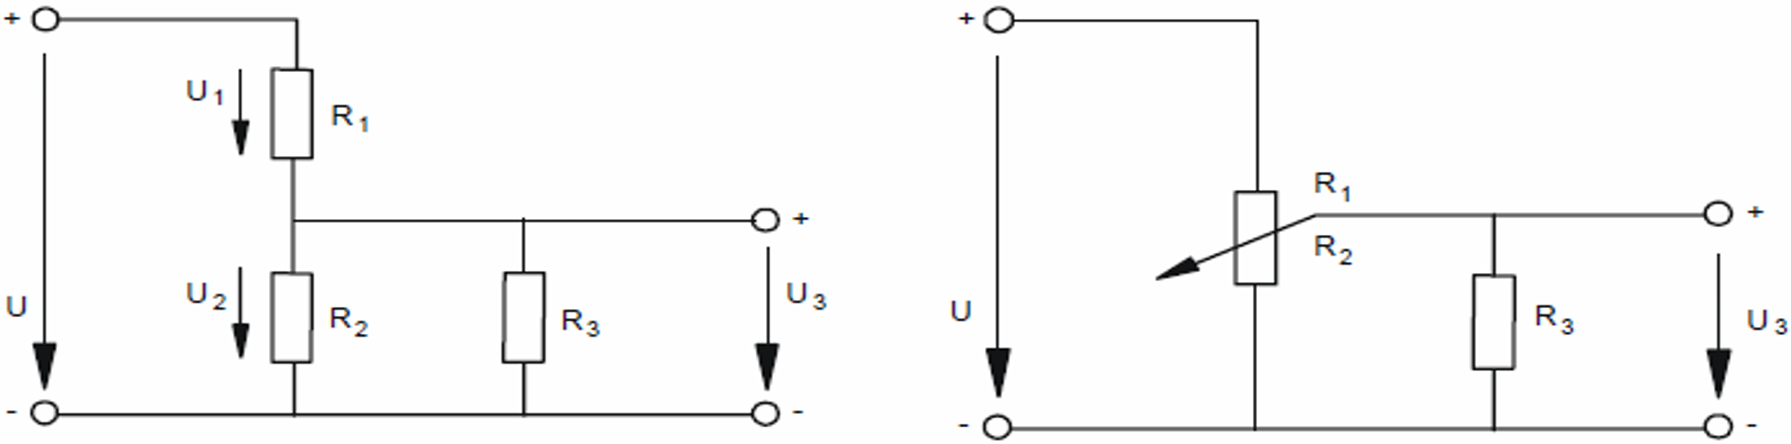
\includegraphics[width=0.8\linewidth]{Pictures/Kapitel5/Belasteter Spannungsteiler 2.png}
    \caption{Belasteter Spannungsteiler}
    \label{fig:K5A1}
\end{figure}

Ein Spannungsteiler besteht aus zwei Widerständen, die in Serie geschaltet sind. Die Ausgangsspannung $U_{out}$ wird über einem der Widerstände abgegriffen. Sobald ein Verbraucher mit Widerstand $R_L$ an die Ausgangsklemmen angeschlossen wird, verändert sich die effektive Last des Spannungsteilers. Die Ausgangsspannung lässt sich nun mithilfe der Ersatzwiderstände berechnen:
\begin{equation} \label{eq:Spannungsteiler2}
    U = U_3 \cdot \frac{R_2 \parallel R_3}{R_1 + (R_2 \parallel R_3)}
\end{equation}
wobei $R_2 \parallel R_3$ der Ersatzwiderstand des parallelen Zweigs ist:
\begin{equation} \label{eq:Parallelschaltung2}
    R_2 \parallel R_3 = \frac{R_2 \cdot R_3}{R_2 + R_3}
\end{equation}

\subsection{Versuchsaufbau}
Für den Versuch wird die in Abbildung~\ref{fig:K5A2} dargestellte Schaltung aufgebaut. Die Eingangsspannung $U_{in}$ beträgt $5\,\unit{V}$, und der Spannungsteiler wird mit einem variablen Widerstand $R = 1\,\unit{\kohm}$ (Potentiometer) realisiert. Zusätzlich wird ein Verbraucherwiderstand $R_3$ parallel zum unteren Teil des Potentiometers geschaltet.

\begin{figure}[H]
    \centering
    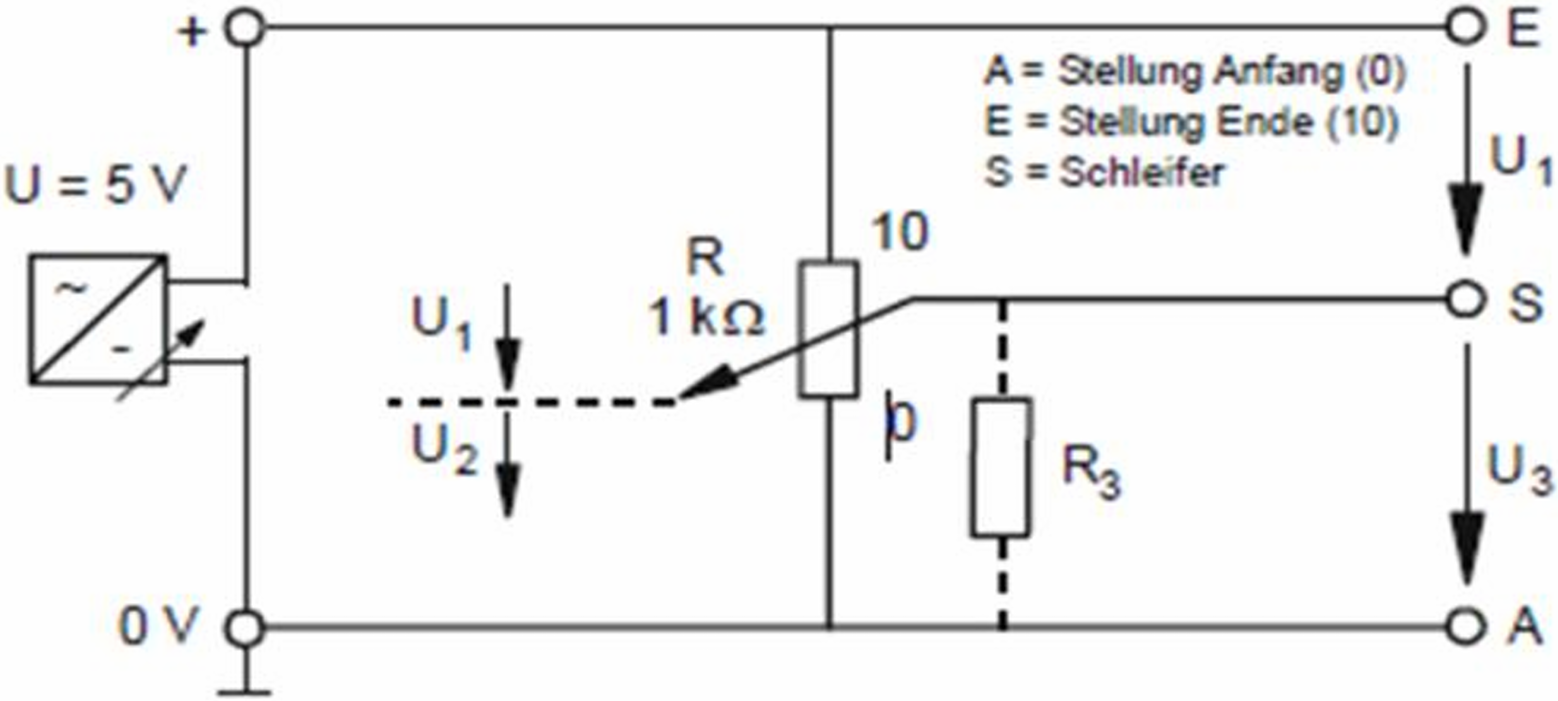
\includegraphics[width=0.6\textwidth]{Pictures/Kapitel5/Belasteter Spannungsteiler.png}
    \caption{Schematischer Aufbau des belasteten Spannungsteilers}
    \label{fig:K5A2}
\end{figure}

\subsection{Versuchsdurchführung}

\begin{enumerate}
    \item Der Spannungsteiler wird so eingestellt, dass die Ausgangsspannung $U_3$ variiert werden kann.
    \item Für jede Einstellung des Potentiometers wird die Spannungen $U_3$ gemessen.
    \item Die Messwerte werden in Tabelle~\ref{tab:K5T1} dokumentiert, grafisch in Form einer Kennlinie in Abbildung~\ref{fig:K5A3} dargestellt und anschließend mit den theoretisch berechneten Werten (siehe Tabelle~\ref{tab:K5T2}) verglichen.
\end{enumerate}

\subsection{Ergebnisse}

Die Messergebnisse des belasteten Spannungsteilers sind in Tabelle~\ref{tab:K5T1} dargestellt:

\begin{table}[H]
\centering
\begin{footnotesize}
\caption{Messwerte des belasteten Spannungsteilers bei Potentiometerstellung $\alpha$.}
\begin{tabular}{c c c c c c c c c c c c}
\toprule
$\alpha$ & 0 & 1 & 2 & 3 & 4 & 5 & 6 & 7 & 8 & 9 & 10 \\
\midrule
$U_3/\,\unit{V}$ $R_3=100\,\unit{\ohm}$ & 0,00 & 0,18 & 0,34 & 0,47 & 0,59 & 0,72 & 0,90 & 1,17 & 1,73 & 2,75 & 4,91\\
$U_3/\,\unit{V}$ $R_3=470\,\unit{\ohm}$& 0,00 & 0,26 & 0,64 & 1,03 & 1,36 & 1,66 & 2,06 & 2,50 & 3,21 & 4,06&4,93 \\
$U_3/\,\unit{V}$ $R_3=1\,\unit{\kohm}$ & 0,00 & 0,27 & 0,73 & 1,23 & 1,67 & 2,04 & 2,50 & 2,97 & 3,64 & 4,32 &4,94 \\
\bottomrule
\end{tabular}
\label{tab:K5T1}
\end{footnotesize}
\end{table}

Die gemessenen Werte stimmen gut mit den berechneten Werten (siehe Tabelle~\ref{tab:K5T2}) überein. Abweichungen sind insbesondere in den unteren Potentiometerstellungen erkennbar, was auf systematische Messfehler oder Widerstandstoleranzen zurückzuführen sein könnte.

\begin{figure}[H]
\centering
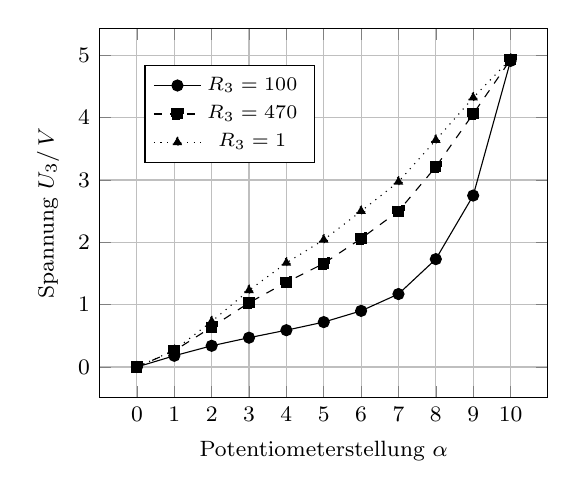
\begin{tikzpicture}
\begin{axis}[
    width=0.6\textwidth,
    xlabel={Potentiometerstellung $\alpha$},
    ylabel={Spannung $U_3/\,\unit{V}$},
    grid=major,
    legend style={at={(0.1,0.9)}, anchor=north west, font=\scriptsize},
    xtick={0,1,2,3,4,5,6,7,8,9,10},
    ytick={0,1,2,3,4,5},
    font=\footnotesize
]

% Daten für R3 = 100 Ohm
\addplot[mark=*,black] coordinates {
    (0,0.00) (1,0.18) (2,0.34) (3,0.47) (4,0.59) (5,0.72) (6,0.90) (7,1.17) (8,1.73) (9,2.75) (10,4.91)};
\addlegendentry{$R_3 = 100\,\unit{\ohm}$}

% Daten für R3 = 470 Ohm
\addplot[mark=square*,black,dashed] coordinates {
    (0,0.00) (1,0.26) (2,0.64) (3,1.03) (4,1.36) (5,1.66) (6,2.06) (7,2.50) (8,3.21) (9,4.06) (10,4.93)};
\addlegendentry{$R_3 = 470\,\unit{\ohm}$}

% Daten für R3 = 1 kOhm
\addplot[mark=triangle*,black,dotted] coordinates {
    (0,0.00) (1,0.27) (2,0.73) (3,1.23) (4,1.67) (5,2.04) (6,2.50) (7,2.97) (8,3.64) (9,4.32) (10,4.94)};
\addlegendentry{$R_3 = 1\,\unit{\kohm}$}

\end{axis}
\end{tikzpicture}
\caption{Kennlinie $U_3 = f(\alpha)$ bei konstanter Eingangsspannung}
\label{fig:K5A3}
\end{figure}

\subsection{Rechnerische Überprüfung}
Die Messwerte werden mit der Gleichung \eqref{eq:Spannungsteiler2} überprüft. Die berechneten Werte sind in Tabelle~\ref{tab:K5T2} dargestellt:

\begin{table}[H]
\centering
\begin{footnotesize}
\caption{Rechnerische Überprüfung der Messwerte des belasteten Spannungsteilers}
\begin{tabular}{c c c c c c c c c c c c }
\toprule
$\alpha$ & 0 & 1 & 2 & 3 & 4 & 5 & 6 & 7 & 8 & 9 & 10 \\
\midrule
$U_3/\,\unit{V}$ $R_3=100\,\unit{\ohm}$ & 0,0 & 0,26 & 0,38 & 0,48 & 0,59 & 0,71 & 0,88 & 1,13 & 1,54 & 2,37 & 5,0 \\
$U_3/\,\unit{V}$ $R_3=470\,\unit{\ohm}$ & 0,0 & 0,42 & 0,75 & 1,04 & 1,32 & 1,63 & 1,99 & 2,42 & 2,98 & 3,78 & 5,0 \\
$U_3/\,\unit{V}$ $R_3=1\,\unit{\kohm}$ & 0,0 & 0,46 & 0,86 & 1,24 & 1,61 & 2,0 & 2,42 & 2,89 & 3,45 & 4,13 & 5,0 \\
\bottomrule
\end{tabular}
\label{tab:K5T2}
\end{footnotesize}
\end{table}

\begin{figure}[H]
\centering
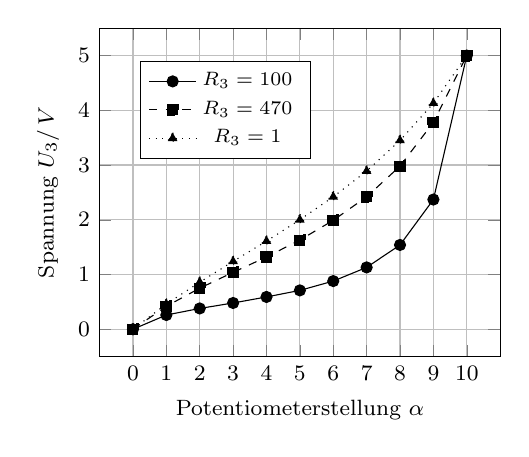
\begin{tikzpicture}
\begin{axis}[
    width=0.55\textwidth,
    xlabel={Potentiometerstellung $\alpha$},
    ylabel={Spannung $U_3/\,\unit{V}$},
    grid=major,
    legend style={at={(0.1,0.9)}, anchor=north west, font=\scriptsize},
    xtick={0,1,2,3,4,5,6,7,8,9,10},
    ytick={0,1,2,3,4,5},
    font=\footnotesize
]

% Daten für R3 = 100 Ohm (aktualisierte Werte)
\addplot[mark=*,black] coordinates {
    (0,0.0) (1,0.26) (2,0.38) (3,0.48) (4,0.59) (5,0.71) (6,0.88) (7,1.13) (8,1.54) (9,2.37) (10,5.0)};
\addlegendentry{$R_3 = 100\,\unit{\ohm}$}

% Daten für R3 = 470 Ohm (aktualisierte Werte)
\addplot[mark=square*,black,dashed] coordinates {
    (0,0.0) (1,0.42) (2,0.75) (3,1.04) (4,1.32) (5,1.63) (6,1.99) (7,2.42) (8,2.98) (9,3.78) (10,5.0)};
\addlegendentry{$R_3 = 470\,\unit{\ohm}$}

% Daten für R3 = 1 kOhm (aktualisierte Werte)
\addplot[mark=triangle*,black,dotted] coordinates {
    (0,0.0) (1,0.46) (2,0.86) (3,1.24) (4,1.61) (5,2.0) (6,2.42) (7,2.89) (8,3.45) (9,4.13) (10,5.0)};
\addlegendentry{$R_3 = 1\,\unit{\kohm}$}

\end{axis}
\end{tikzpicture}
\caption{Kennlinie der theoretischen Werte $U_3 = f(\alpha)$ bei konstanter Eingangsspannung.}
\label{fig:K5A4}
\end{figure}


\subsection{Diskussion und Interpretation}
Die Ergebnisse verdeutlichen den Einfluss des parallel geschalteten Verbraucherwiderstands $R_3$ auf die Ausgangsspannung $U_3$ des Spannungsteilers. Im Vergleich zum unbelasteten Fall, bei dem der Spannungsteiler nur aus den Widerständen $R_1$ und $R_2$ besteht, führt die zusätzliche Belastung durch $R_3$ zu einer Verringerung der effektiven Ausgangsspannung. Diese Verringerung ist umso ausgeprägter, je kleiner der Wert von $R_3$ ist. 

Die theoretischen Werte zeigen, dass bei \(R_3 = 100\,\unit{\ohm}\) die Belastung deutlich stärker ausfällt als bei \(R_3 = 470\,\unit{\ohm}\) oder \(R_3 = 1\,\unit{\kohm}\). Dies liegt daran, dass der Ersatzwiderstand $R_2 \parallel R_3$ mit sinkendem $R_3$ ebenfalls sinkt, was den Spannungsabfall am oberen Widerstand $R_1$ erhöht und die Ausgangsspannung verringert.

Darüber hinaus wird festgestellt, dass die Abweichungen zwischen den gemessenen und theoretischen Werten in den niedrigen Potentiometerstellungen (\(\alpha \leq 4\)) am größten sind. Diese Abweichungen können durch folgende Faktoren erklärt werden:
\begin{itemize}
    \item Kontaktwiderstände: An den Anschlüssen des Potentiometers können zusätzliche Widerstände auftreten, die den Gesamtwiderstand beeinflussen.
    \item Toleranzen der Widerstände: Kommerzielle Widerstände haben typischerweise eine Toleranz von 1\% bis 5\%, die die Ergebnisse insbesondere bei kleinen Widerstandswerten stark beeinflussen können.
    \item Messgeräteungenauigkeiten: Die Genauigkeit der verwendeten Multimeter und deren Kalibrierung spielen eine wichtige Rolle, insbesondere bei niedrigen Spannungen.
    \item Systematische Fehler: Der Aufbau der Schaltung kann zusätzliche Verluste verursachen, beispielsweise durch Leitungswiderstände oder nicht ideale Kontakte.
\end{itemize}

Eine interessante Beobachtung ist die Nichtlinearität des Spannungsverlaufs bei hohen Potentiometerstellungen (\(\alpha > 7\)). In diesem Bereich wird $R_2$ dominant, und der Ersatzwiderstand $R_2 \parallel R_3$ nähert sich dem Wert von $R_3$. Dadurch wird der Spannungsabfall am Verbraucher geringer, was zu einem flacheren Anstieg der Kennlinie führt.

Der belastete Spannungsteiler findet breite Anwendung in der Elektronik, insbesondere bei Spannungsteilerregelungen und Signalabschaltungen. Das Verständnis der Belastung ist entscheidend, um eine korrekte Dimensionierung der Widerstände und Verbraucher sicherzustellen. Ein häufiges Beispiel ist die Anpassung von Spannungssignalen an analoge oder digitale Eingänge, bei denen die Eingangsimpendanz des Folgeschaltkreises als Verbraucher wirkt.

Um die Auswirkungen der Belastung weiter zu untersuchen und die Ergebnisse zu optimieren, könnten folgende Maßnahmen durchgeführt werden:
\begin{itemize}
    \item Einsatz präziser Widerstände: Verwendung von Widerständen mit geringere Toleranzen, beispielsweise 0,1\%.
    \item Vermeidung von Kontaktwiderständen: Verwendung hochwertiger Kontaktstellen und feste Lötverbindungen anstelle von Steckverbindern.
    \item Erhöhung der Eingangsspannung: Dies würde die Messung bei niedrigen Spannungen präziser machen, da relative Fehler reduziert werden.
\end{itemize}

Zusammenfassend zeigt der Versuch die Bedeutung einer genauen Analyse von belasteten Spannungsteilern in der Elektrotechnik. Die Erkenntnisse sind von grundlegender Bedeutung für die Dimensionierung und Optimierung elektronischer Schaltungen.


\newpage